%%%%%%%%%%%%%%%%%%%%%%%%%%%%%%%%%%%%%%%%%%%%%%%%%%%%%%%%%%%%%%%%%%%%%%%%%
%
%	LaTeX File for Stanford University PhD Thesis
%
%%%%%%%%%%%%%%%%%%%%%%%%%%%%%%%%%%%%%%%%%%%%%%%%%%%%%%%%%%%%%%%%%%%%%%%%%
%	Copyright 2001  by  Jung-Suk Goo    (goojs@gloworm.stanford.edu)
%%%%%%%%%%%%%%%%%%%%%%%%%%%%%%%%%%%%%%%%%%%%%%%%%%%%%%%%%%%%%%%%%%%%%%%%%

\chapter{Introduction}
\label{chap:intro}

%%%%%%%%%%%%%%%%%%%%%%%%%%%%%%%%%%%%%%%%%%%%%%%%%%%%%%%%%%%%%%%%%%%%%%%%
\fancypar{T}{{\sc his file}} is the introduction.

\cite{abidi:ieee_ted86}
\cite{cheng:em}
\cite{mesh:book}
\cite{biber:mtt_s98}
\cite{atn:np5b}

\begin{figure}[t]
        \centering
        \subfigure[]{\includegraphics[width=.270\linewidth]
                                {FIGURES/figure1.eps}}
        \hspace{0.10\linewidth}
        \subfigure[]{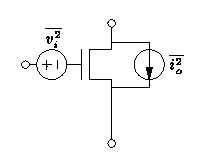
\includegraphics[width=.290\linewidth]
                                {FIGURES/figure2.eps}}
        \caption{MOSFET thermal noise models.
                (a) van der Ziel model
                (b) Pospieszalski Model.}
        \label{F:goo:noise_model1}
\end{figure}
